\documentclass[12pt]{article}
\usepackage{amsmath}
\usepackage{amssymb}
\usepackage{graphicx}
\usepackage{hyperref}
\usepackage{cleveref}
\usepackage[most]{tcolorbox}
\usepackage[utf8]{inputenc}
\usepackage{tikz}
\usepackage{pstricks-add}
\usepackage{centernot}
\usepackage{enumerate}
\usepackage{MnSymbol}
\usepackage{mathtools}
\usepackage{subcaption}
\usepackage{geometry}
 \geometry{
 a4paper,
 total={170mm,257mm},
 left=20mm,
 top=20mm,
 }
\DeclarePairedDelimiter\ceil{\lceil}{\rceil}
\DeclarePairedDelimiter\floor{\lfloor}{\rfloor}
\DeclarePairedDelimiter\abs{\left|}{\right|}
\hypersetup{
    colorlinks=false,
    pdfborder={0 0 0},
}
\newcommand\tab[1][1cm]{\hspace*{#1}}
\newtheorem{theorem}{Theorem}
\newtheorem{corollary}{Corollary}
\usetikzlibrary{arrows,calc}
\title{MAT 1001: Calculus I}
\author{Alfonsus Rodriques Rendy}
\date{2021-9-30}

\begin{document}
\begin{center}
    \hspace*{-0.5cm}
    \framebox{
    \begin{minipage}{1\linewidth}
        \textbf{MAT1001 Calculus I} \\
        \vspace{-0.8cm}
        \begin{center}
            \huge{Lecture 7 - 11 : Applications of Derivative} 
            \\
            \vspace{0.5cm}
            \normalsize \textit{Lecture by Dr. Arjan Abeynaike} \\
            \vspace{0.3cm}
            \text{Scribe by Alfonsus Rodriques Rendy} \\
            \textrm{Sep 30, 2021 - Oct 19, 2021}
        \end{center}
    \end{minipage}}
\end{center}

\section{Extreme Values of Function}
\paragraph{Definition}
Let $f$ be a function with domain $D$. Then $f$ has an \textbf{absolute maximum} value on $D$ at a point $c$ if
\[
    f(x) \leq f(c), \forall\: x \in D
\]
and an \textbf{absolute minimum} value on $D$ at $c$ if
\[
    f(x) \geq f(c), \forall\: x \in D
\]
Maximum and minimum values are called \textbf{extreme values} of the function $f$. 
Absolute maxima or minima are global maxima or minima. \\ 
Maxima and Minima = Extrema = Plural of Extremum / Maximum and Minimum

\begin{theorem}[Extreme Values Theorem] 
    If $f$ is continuous on a closed interval $[a, b]$ , then $f$ attains both an absolute maximum 
    value $M$ and an absolute minimum value $m$ in $[a, b]$ . That is, there are numbers $x_1$ and $x_2$ in $[a, b]$
    with 
    \[
        f(x_1) = m,\: f(x_2) = M\: \textrm{, and } m \leq f(x) \leq M\quad \forall\: x \in [a, b] \setminus x_1, x_2
    \]
    \label{extreme value}
\end{theorem}
\paragraph{Note} The requirement of extreme values theorem is \textbf{continuous function} and \textbf{defined in a closed interval}

\paragraph{Example} Find the absolute maximum and minimum of the graph $y = x^2$ on (a) its domain, (b) in $[0, 2]$, (c) in $(0, 2]$, (d) in $(0, 2)$!

\begin{figure}[h!]
    \centering
    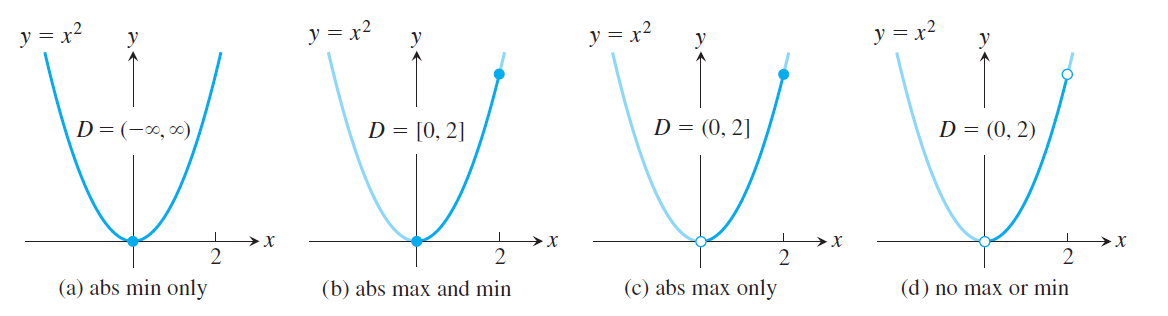
\includegraphics[width=1\linewidth]{Images/absolute max min.png}
    \caption{Absolute maximum and minimum of $f(x) = x^2$ on different interval}
\end{figure}

\noindent 
(a) $x \in D = \mathbb{R}$ : Absolute Maximum = None, Absolute Minimum = 0 at $x = 0$ \\
(b) $x \in [0, 2]$ : Since, $f(x)$ is continuous and defined on a closed interval $[0, 2]$, the extreme values theorem guarantees that it has absolute maximum and minimum,
that is: \\
Absolute Maximum = 4 at $x = 2$ Absolute Minimum = 0 at $x = 0$ \\
(c) $x \in (0, 2]$ : Absolute Maximum = None, Absolute Minimum = None \\
(d) $x \in (0, 2)$ : Absolute Maximum = None, Absolute Minimum = None 

\paragraph{Definition}
A function $f$ has a \textbf{local maximum} value at $a$ point $c$ within its
domain $D$ if 
\[ 
    f(x) \leq f(c)\: \forall\quad x \in (c - \delta, c + \delta) \cap D
\]

\noindent 
A function $f$ has a \textbf{local minimum} value at $a$ point $c$ within its domain $D$ if
\[ 
    f(x) \geq f(c)\: \forall\quad x \in (c - \delta, c + \delta) \cap D
\]

\begin{figure}[h!]
     \centering
     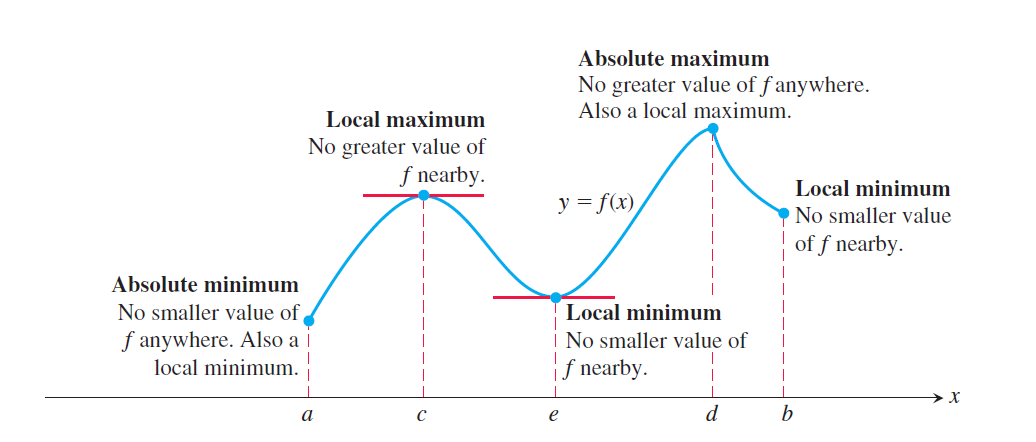
\includegraphics[width=1\linewidth]{Images/absolute and local extrema.png}
     \caption{Illustration of local vs absolute extrema}
\end{figure}

\paragraph{Definition:  Critical Points}
Let $f : D \to \mathbb{R}$, and let $c$ be an interior point of $D$. Then $c$ is a critical point of $f$ if:
\begin{enumerate}[i]
    \item $f'(c) = 0$ 
    \item $f'(c)$ does not exist ($f'(c) \notin \mathbb{R})$
\end{enumerate}

\paragraph{Example} What are all the critical points of the function 
\begin{align*} 
    f(x) = 
    \begin{cases} 
        |x| & x <  1 \\
        1 & x \geq 1
    \end{cases}
\end{align*}

\noindent
(i) $f'(x)$ is not defined at $x = 0$, so 0 is a critical point. \\
(ii) $f'(x)$ = 0 at $x \geq 1$, so $x \geq 1$ is critical points. 

\noindent
Hence, critical points = ${0} \cup [1, \infty]$

\begin{theorem}[The First Derivative Theorem of Local Extrema]
    If $f$ has a local maximum or minimum value at an interior point $c$ of its domain,
    and if $f'(x)$ is defined at $c$, then $f'(x) = 0$ \\

    \noindent
    or let $c$ be an interior point of $D$. If a function $f : D \to \mathbb{R}$ has a local extrema
    at $c$, then $c$ is a critical point of $f$.
    \label{local extrema}
\end{theorem}

\paragraph{Note} Note that the converse of theorem \ref{local extrema} is not true, that is critical point $\nRightarrow$ extrema. The counterexample
is $f(x) = x^3$

\paragraph{Finding Local Extrema}
We can use theorem \ref{extreme value} and theorem \ref{local extrema} to help us find all local extrema and global extrema of $f(x)$ defined in closed interval $x \in [a, b]$, that is:
(1) Evaluate all critical points and endpoints, (2) Take the largest and smallest of these value to be global extrema.

\paragraph{Example} Find all the absolute extreme (with values and positions) of
\[
    f : [ -2,4] \to \mathbb{R} \textrm{\tab \tab} f(x) = 2x^3 - 3x^2 - 12x + 15
\]

\noindent
(1) Find all Critical values and Endpoints
\[
    f'(x) = 6x^2 - 6x - 12
\]


First, $f'(x) = 0$ :
\begin{align*} 
    6x^2 - 6x - 12 &= 0 \\
    6(x - 2)(x + 1) &= 0
\end{align*}

$x = {-1, 2}$ \\

Then, find x when $f'(x)$ doesn't exists. Since $f'(x) = 6x^2 - 6x - 12$ is defined on $D \in \mathbb{R}$, Then
for all $x \in \mathbb{R}$,  $f'(x)$ exists. \\

Endpoints are $x = {-2, 4}$, so all possible $x$ are: $x = {-2, -1, 2, 4}$. \\

\noindent
(2) Find the largest and smallest \\
$f(-2) = 11$, $f(-1) = 22$, $f(2) = -5$, $f(4) = 47$.\\
Hence, absolute maximum point = (4, 47) and absolute minimum point = (2, -5) 

\paragraph{Proof of theorem \ref{local extrema}}
Suppose that $f$ has a local maximum at $c$ (the case where  $c$ gives a minimum is  similar).
Then 
\[ 
    \exists \; a > 0\textrm{ s.t. } f(c) \geq f(x) \;  \forall \; x \in (c - a, c + a)
\]

\noindent
Let
\[
    g(x) = \frac{f(x) - f(c)}{x - c} 
\]
for 
\[
    x \in (c - a, c + 1) \setminus {c} 
\]

(i) For $x \in (c - a, c)$ 
\[
    f(x) - f(c) \leq 0 \textrm{ \tab and \tab} x - c < 0 \textrm{\tab} \Rightarrow \textrm{\tab} g(x) \geq 0
\]
Based on theorem 9 in lecture 2 (the inequality of limit), we have
\[
    \lim_{x \to c^{ -}} g(x) \geq \lim_{x \to c^{ - }} 0 = 0
\]

(ii) For $x \in (c, c + a)$ 
\[
    f(x) - f(c) \leq  0 \textrm{ \tab and \tab} x - c > 0 \textrm{\tab} \Rightarrow \textrm{\tab} g(x) \leq  0
\]
Based on theorem 9 in lecture 2 (the inequality of limit), we have
\[
    \lim_{x \to c^{ + }} g(x) \leq  \lim_{x \to c^{ + }} 0 = 0
\]

\noindent
Since $f'(x)$ is defined on c $f^{'}_{-} (x) = f^{'}_{+} (x) = f'(x)$, So
\[
    0 \leq \lim_{x \to c^{ - }} g(x) = f^{'}_{-} (x) = f'(x) = f^{'}_{+} (x) = \lim_{x \to c^{ + }} g(x) \leq 0
\]
Hence, $f'(x) = 0$

\section{Rolle's Theorem}
\begin{theorem}[Rolle's Theorem] 
    Suppose that a function $f$ is continuous on $[a, b]$ and differentiable at every point in $(a, b)$, and it satisfies $f(a) = f(b)$.
    Then there exists $c$ in $(a, b)$such that $f'(c) = 0$.
\end{theorem}

\begin{figure}[h!]
     \centering
     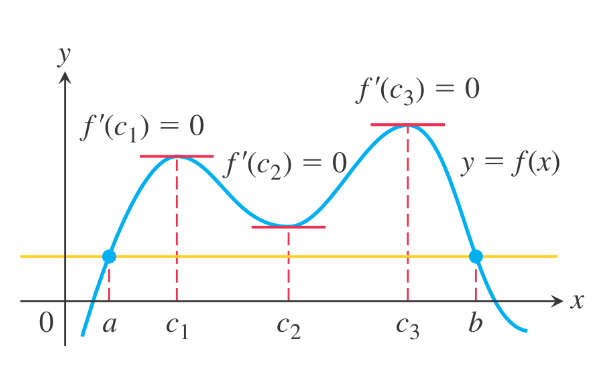
\includegraphics[width = 0.5\linewidth]{Images/rolle's theorem.png}
     \caption{Illustration of Rolle's theorem. }
\end{figure}

\paragraph{Proof}
By Extreme Value Theorem, there must exists $c_1, c_2 \in [a,b]$ such that $f(c_1) = m$ and $f(c_2) = M$, where 
$m$ and $M$ are absolute minimum and maximum respectively.  \\

\noindent
(i) If $m = M$, then $f(x) = M \; \forall x \in [a, b]$, so $f'(c) = 0$ for any $c \in (a, b)$.  \\
(ii) Suppose $m < M$ then either $f(a) = f(b) \neq m$ or $f(a) = f(b) \neq M$. One or bot must holds true. So:

(1) $f(a) = f(b) \neq m \Rightarrow \: \exists \: c_1 \in (a,b) $ s.t. $f(c_1) = m$ 

(2) $f(a) = f(b) \neq M \Rightarrow \: \exists \: c_2 \in (a,b) $ s.t. $f(c_2) = M$ \\

\noindent
Since $f(c_1)$ and $f(c_2)$ is defined in both cases, then by theorem \ref{local extrema}, $f'(c_1)$ and $f'(c_2)$ = 0. Hence, rolle's theorem
holds on both cases with $c = c_1$ and $c = c_2$ respectively.

\paragraph{Intuition}
If an object moves and the final position on $t = b$ is the same as the start position on $t = a$, then we can conclude that
there must exists $t \in (a, b)$ such that the velocity of the object is 0.

\paragraph{Example}
Show that the equation $x^3 + 3x + 1 = 0$ has exac

\paragraph{Solution}
Let $f(x) = x^3 + 3x + 1$.

\[
  f(-1) = - 3 \textrm{\tab and \tab} f(0) = 1  
\]

Since $f(x)$ is continuous and $f(x) \in [-3, 1]$ for $x \in [-1, 0]$, there must
exists $f(c) = 0$ with $c \in (-1, 0)$.

\[
    f'(x) = 3x^2 + 3
\]

Since $f'(x) > 0$ for all $x \in \mathbb{R}$ then the $f(x)$ is strictly increasing 
(no critical point). So, there is only one solution of $x^3 +3x + 1$.

\section{The Mean Value Theorem}
\subsection{Theorem and Proof}
\begin{theorem}[Mean Value Theorem]
    Suppose that a function $f$ is continuous on $[a, b]$ and differentiable on $(a, b)$. 
    Then there exists $c$ in $(a, b)$ such that:
    \[
        f'(c) = \frac{f(b) - f(a)}{b - a} 
    \]
\end{theorem}

\begin{figure}[h!]
     \centering
     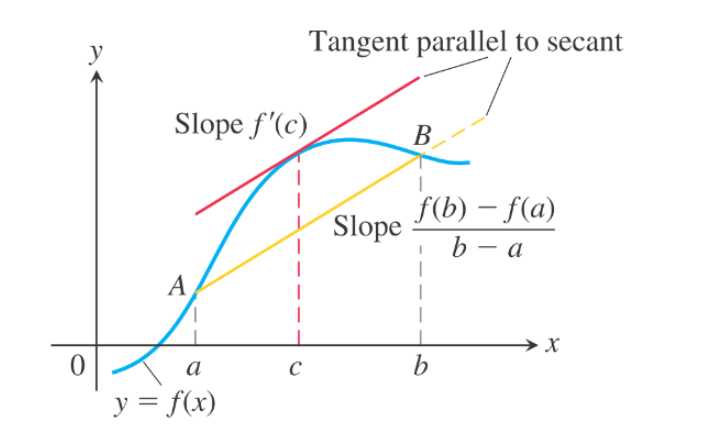
\includegraphics[width = 0.5\linewidth]{Images/mvt.png}
     \caption{There exists a tangent line in $(a, b)$ that have the same gradient
     with the secant line on $(a, b)$}
\end{figure}

\paragraph{Proof}
First we define $h(x)$ on $[a,b]$ as
\[
  h(x) = f(x) - ((f(a) + \frac{f(b) - f(a)}{b - a}(x - a) ))\, 
\]
\begin{figure} [h!]
    \centering
    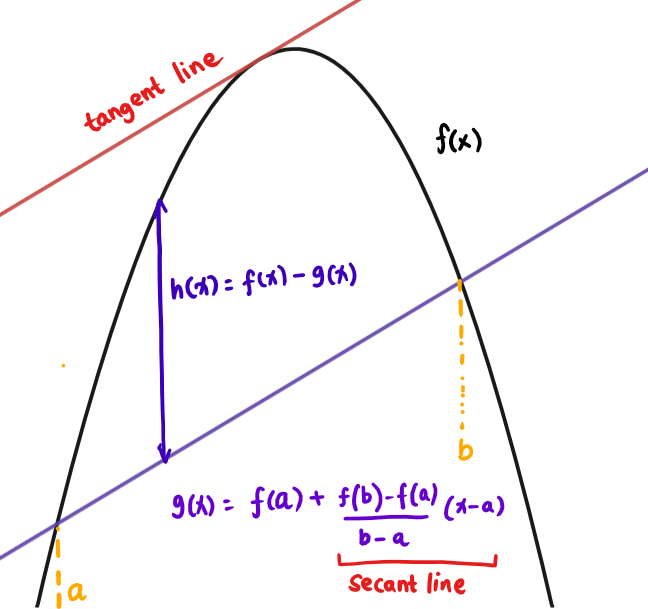
\includegraphics[width = 0.35\linewidth]{Images/mvt proof.png}
    \caption{Illustration of $h(x)$}
\end{figure}
Hence, $h(a) = h(b) = 0$ (see from the graph).

Since $h$ is continuos on $[a,b]$ and differentiable on $(a,b)$, then by 
Rolle's theorem there exists $c \in (a,b)$ such that $h'(c) = 0$

\begin{align*} 
     h'(x) &= f'(x) - \frac{f(b) - f(a)}{b - a}  \textrm{\tab} \forall x \in (a,b)\\
    0 &= f'(x) - \frac{f(b) - f(a)}{b - a}\\
    f'(x) &= \frac{f(b) - f(a)}{b - a} \\
\end{align*}

\subsection{Consequences and Corollary}
\paragraph{Physical Consequence}
Suppose that $f(t)$ represents the distance travelled until time $t$.Then the mean value 
theorem implies that if we pick two moments $t = a$ and $t = b$, there has to be some moment 
$t = c$ in between at which the instantaneous speed is equal to the average speed between $t = a$ and $t = b$.

\begin{corollary}[MVT] 
     If $f'(x) = 0$ at each point of $x$ of an open interval  $(a,b)$ then $f(x) = C$ 
     for all $x \in (a,b)$ where $C$ is a constant.
\end{corollary}

\paragraph{Proof}
Let $x_1, x_2 \in (a,b)$. From MVT we know that 
\[
    f'(c) = \frac{f(x_2) - f(x_1)}{x_2 - x_1} 
\]
with $c \in (a,b)$. Then, if $f'(c) = 0$
\[
    0 = \frac{f(x_2) - f(x_1)}{x_2 - x_1} 
\]
Hence, if $f'(x) = 0 \; \forall \: x \in (a,b)$:
\[
    f(x_2) = f(x_1) = C \textrm{\tab} \forall x \in (a, b)
\]

\begin{corollary}[MVT] 
     If $f'(x) = g'(x)$ at each point $c$ of an open interval $(a,b)$ then there exists
     a constant $C$ such that $f(x) = g(x) + C$ for all $x \in (a,b) $, or $f - g$ is a constant 
     for all $x \in (a,b)$. 
\end{corollary}

\begin{figure}[h!]
     \centering
     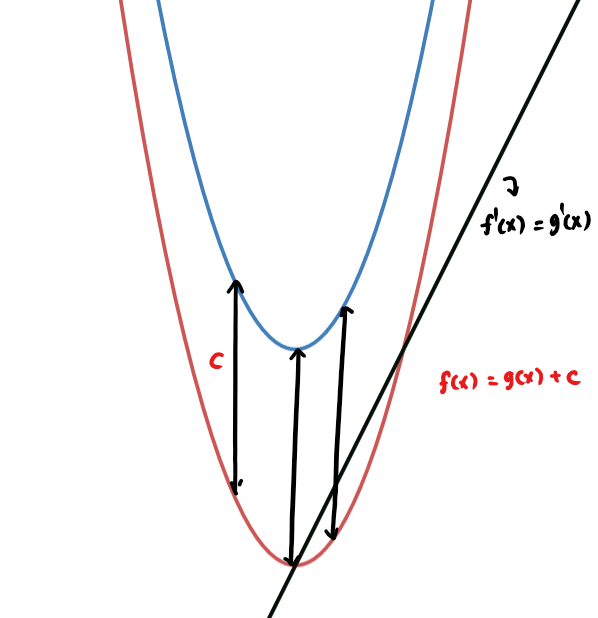
\includegraphics[width = 0.35\linewidth]{Images/corollary 2.png}
\end{figure}
\paragraph{Proof}
Let $h(x) = f(x) - g(x)$ then
\[
    h'(x) = f'(x) - g'(x) = 0
\]
\noindent
By corollary MVT 1:
\[
    h(x) = f(x) - g(x) = C \textrm{\tab} \forall \, x \in (a,b)
\]

\paragraph{Example 1} If $f'(x) = \sin x$ then what is $f(x)$? \\

We know that if $g(x) = - \cos x$ then $g'(x) = sin (x) = f'(x)$ $\forall x$.
Hence $f(x) = - \cos x + C$ with C is a constant. 

\paragraph{Note} This concept is called antiderivative and will be covered later.

\paragraph{Example 2} Prove that
\[
    | \sin (x) - \sin (y)| \leq |x - y| \; \forall \, x, y \in \mathbb{R}
\]

(i) For the case $x = y$ then both sides = 0, hence it's proven \\ 
(ii) For the case $x \neq y$, let $y < x$. \\
Let $f(z) = sin(z)$. Since $\sin z$ is differentiable and continuous for all $x \in \mathbb{R}$, by MVT there exists:
\begin{align*} 
    f'(c) &= \frac{f(x) - f(y)}{x - y} \\
    \cos (z) &=  \frac{f(x) - f(y)}{x - y} \\
\end{align*}

Since $-1 \leq \cos z \leq 1$, then
\begin{align*} 
    \left|\frac{\sin x - \sin y)}{x - y} \right| &\leq 1 \\
    \left|\:  \sin x - \sin y\: \right| &\leq |x - y| \\
\end{align*}
    
\section{Monotonicity}
\subsection{Definition and Corollary}
\paragraph{Definition} Let $f$ be a function defined on an interval $I$ and let $x_1$ and $x_2$ be any two points in $I$.
\begin{enumerate} 
     \item If $f(x_2) > f(x_1)$ whenever $x_1 < x_2$ then $f$ is said to be \textbf{increasing}
     \item If $f(x_2) < f(x_1)$ whenever $x_1 < x_2$ then $f$ is said to be \textbf{decreasing}
\end{enumerate}
A function that is increasing or decreasing on $I$ is said to be \textbf{monotonic} on $I$.

\begin{corollary}[Monotonicity]
    Suppose that a function $f$ is continuous on $[a, b]$ and differentiable on $(a,b)$.
    \begin{enumerate} 
        \item If $f'(x) > 0$ for all $x \in (a,b)$, then $f$ is increasing on $[a, b]$
        \item If $f'(x) < 0$ for all $x \in (a,b)$, then $f$ is decreasing on $[a, b]$
   \end{enumerate}
\end{corollary}

\paragraph{Proof (1)}
Let $x_1, x_2 \in [a, b]$ and $x_1 < x_2$. Since $f$ is continuous on $[x_1, x_2]$ and differentiable
on $(x_1, x_2)$, by MVT there exists $c \in (x_1, x_2)$ such that
\[
    f(x_2) - f(x_1) = f'(c)(x_2 - x_1)
\]
Since $x_2 - x_1 > 0$, and $f'(c) > 0$ then we have
\[
  f(x_2) - f(x_1) > 0
\]
Hence, $f(x_2) > f(x_1)$ with $x_1 < x_2$, and by definition $f$ is increasing on $[a, b]$

\paragraph{Proof (2)}
Let $x_1, x_2 \in [a, b]$ and $x_1 < x_2$. Since $f$ is continuous on $[x_1, x_2]$ and differentiable
on $(x_1, x_2)$, by MVT there exists $c \in (x_1, x_2)$ such that
\[
    f(x_2) - f(x_1) = f'(c)(x_2 - x_1)
\]
Since $x_2 - x_1 > 0$, and $f'(c) < 0$ then we have
\[
  f(x_2) - f(x_1) < 0
\]
Hence, $f(x_2) < f(x_1)$ with $x_1 < x_2$, and by definition $f$ is decreasing on $[a, b]$

\paragraph{Example} Prove that $f(x) = \sqrt(x)$ is increasing on $(0, \infty)$. \\
First,
\[
  f'(x) = \frac{1}{2\sqrt{x}}\, 
\]
Since $f'(x) > 0 \; \forall \, x \in [0, \infty]$ then by corollary 3 (monotonicity), $f(x)$ is increasing
on $[0, b]$ with $b \in \mathbb{R}$. Hence, $f$ is increasing on $[0, \infty)$.
\subsection{Interval of Monotonicity}
\paragraph{Definition}
Suppose that $x_1, x_2, ..., x_n$ are all critical points of a function $f$, with $x_1 < x_2 < ... < x_n$.
Let $x_i$ and $x_{i+1}$ be two consecutive critical points. If $f'$ is continuous on $[x_i, x_{i + 1}]$, 
then $f'$ is either entirely positive or entirely negative on $(x_i, x_{i+1})$. Hence, by corollary monotonicity (3):
\begin{enumerate} 
    \item $f$ is increasing on $[x_i, x_{i+1}]$ if $f'(c) > 0$ for some $c \in (x_i, x_{i+1})$
    \item $f$ is decreasing on $[x_i, x_{i+1}]$ if $f'(c) < 0$ for some $c \in (x_i, x_{i+1})$
\end{enumerate}
Similar statements can be made about the intervals $(-\infty, x_1)$ and $(x_n, \infty)$.

\paragraph{Example} Let $f(x) = x^3 - 12x + 5$, determine the intervals of monotonicity!
\[
    f'(x) = 3x^2 - 12 = 3(x + 2)(x - 2)
\]
We have critical points $c = \{-2, 2\}$
Hence, the intervals of monotonicity is $(-\infty, -2), (-2, 2), (2, \infty)$ 
\section{Derivative Test}
\subsection{First Derivative Test}
Suppose $c$ is a critical point of a continuous function $f$ that is differentiable at 
every point in an interval containing $c$ except possibly at $c$, then if we move from left to right 
of the function:
\begin{enumerate} 
     \item If $f'$ changes from negative to positive at $c$, then $c$ is a local minimum.
     \item If $f'$ changes from positive to negative at $c$, then $c$ is a local maximum.
     \item If $f'$ doesn't change then $f$ has no extremum at $c$.
\end{enumerate}
In other words:
\begin{enumerate} 
    \item $\exists \, a > 0 : f'(x) < 0 \; \forall \, x \in (c - a, c) \textrm{ and }  f'(x) > 0 \; \forall x \in (c, c + a)$, $c$ is a local minimum
    \item $\exists \, a > 0 : f'(x) > 0 \; \forall \, x \in (c - a, c) \textrm{ and }  f'(x) < 0 \; \forall x \in (c, c + a)$, $c$ is a local maximum
    \item $\exists \, a > 0 : f'(x) > 0 \textrm{ or } f'(x) < 0 \; \forall \, x \in (c - a, c + 1)$
\end{enumerate}

\begin{figure}[h!]
    \centering
    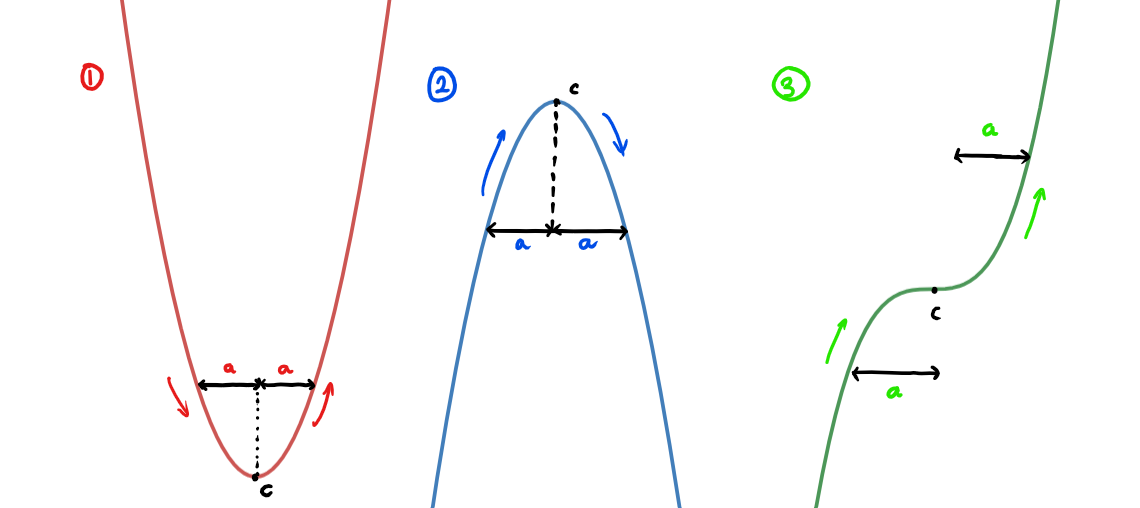
\includegraphics[width = 0.8\linewidth]{Images/first derivative test.png}
    \caption{First derivative test (1) Minimum point, (2) Maximum point (3) Neither}
\end{figure}
\paragraph{Proof (1)}
By corollary (3) of monotonicity, $f$ is decreasing on $[c - a, c]$ and increasing on 
$(c, c + a]$ which means $f(c) < f(x) \; \forall \, x \in [c - a, c)$ and $f(c) < f(x) \; \forall
\, x \in (c - a, c + a) \setminus\{c\}$. Hence, by definition $f$ has a local minimum at $c$.

\paragraph{Example}
Find all absolute and local extrema for $f(x) = x^{4/3} - 4x^{1/3}$
\[
    f'(x) = \frac{4}{3}x^{ - \frac{2}{3}}(x - 1)
\]
$f'(x) = 0$ when $x = 1$ and $x = 0$
For $x = 0$
\[
    \lim_{h \to 0} \frac{f(x) - f(0)}{h} = \frac{h^{\frac{4}{3}} - 4h^{ - \frac{1}{3}}}{h} = h^{\frac{1}{3}} - 4h^{ - \frac{2}{3}} = DNE 
\]
Hence, $f'(x)$ is not defined.
Then we have - - - |0|- - - |1| +++. By first derivative test, $f(x)$ has a local minimum point at $x = 1$. Since $x \to \pm \infty$ f(x) is increasing,
then $x = 1$ is also an absolute minimum.
\subsection{Concavity and Inflection Point}
\paragraph{Definition - Concavity}
The graph of a differentiable function $y = f(x)$ is:
\begin{enumerate} 
     \item \textbf{Concave up} on an interval $I$ if $f'(x)$ is increasing.
     \item \textbf{Concave down} on an interval $I$if $f'(x)$ is decreasing.
\end{enumerate}
\begin{figure}[h!]
     \centering
     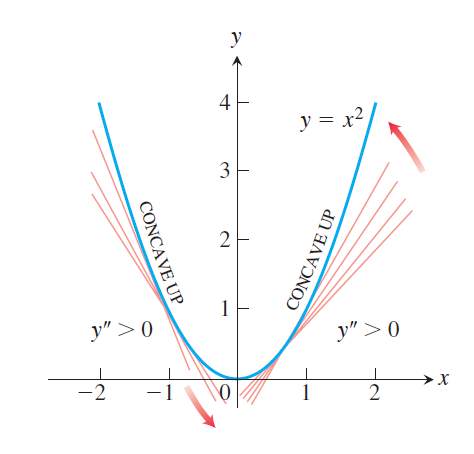
\includegraphics[width = 0.4\linewidth]{Images/concavity.png}
     \caption{Function Concavity}
\end{figure}

\paragraph{Second Derivative Test of Concavity}
Suppose $y = f(x)$ is a twice differentiable function on an interval $I$ then
\begin{enumerate} 
     \item If $f''(x) > 0$ on $I$, the graph $f$ on $I$ is concave up 
     \item If $f''(x) < 0$ on $I$, the graph $f$ on $I$ is concave down
\end{enumerate}
\paragraph{Proof (1)}
Suppose $f''(x) > 0 \; \forall \, x \in I$. Then, by corollary (3) $f'(x)$ is increasing on $I$. Hence, $f$ is concave up.
\paragraph{Example} Find the concavity of $y = x^3$ 
\begin{align*} 
     f'(x) = 3x^2 \\
     f''(x) = 6x 
\end{align*}
So, $f''(x) > 0$ if $x > 0$ and $f''(x) < 0$ if $x < 0$.

\paragraph{Definition - Inflection Point} is a point $(c, f(c))$ where $f(x)$ has a tangent line and where the concavity changes.
If $c$ is an inflection point, then either $f''(c) = 0$ or $f''(x)$ doesn't exist. However, $f''(c) = 0$ doesn't imply that $c$ is an inflection point.
\paragraph{Note} In Thomas' Calculus, an inflection point need to have \textbf{a tangent line} or differentiable at $c$.
\begin{figure}[h!]
    \centering
    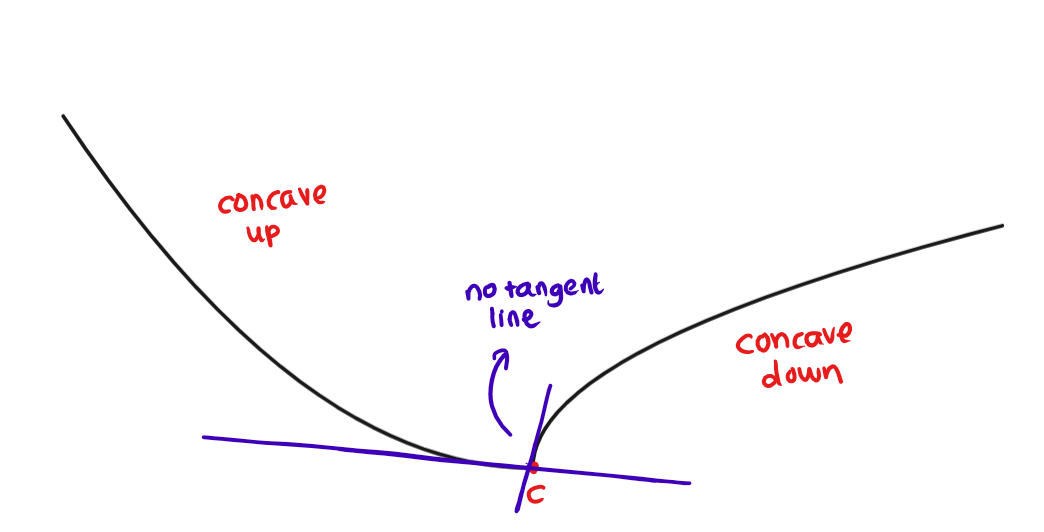
\includegraphics[width = 0.6\linewidth]{Images/inflection fail.png}
    \caption{Where inflection point fails, at $c$, $f(x)$ doesn't have a tangent line}
\end{figure}
\paragraph{Example} Find the inflection point of $f(x) = x^{1/3}$
\[
    f'(x) = \frac{1}{3}x^{ - \frac{2}{3}}, f''(x) = - \frac{2}{9} x^{ - \frac{5}{3}}
\]
At $x = 0$, $f'(x)$ and $f''(x)$ doesn't exist.
\[
    \lim_{x \to 0} f'(x) = \frac{1}{3 \sqrt[3]{x^2}} = + \infty
\]
Hence, $f(x)$ has a tangent line at $x = 0$.
\begin{align*} 
     f''(x)
     \begin{cases} 
        > 0 \; x < 0 \\
        < 0 \; x > 0 \\
    \end{cases} 
\end{align*}

\begin{figure}[h!]
     \centering
     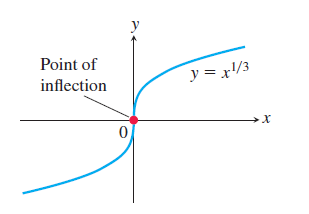
\includegraphics[width = 0.5\linewidth]{Images/inflection example.png}
     \caption{Graph of $y = x^{1/3}$}
\end{figure}
Hence, (0,0) is a point of inflection.


\subsection{Second Derivative Test}
\paragraph{Second derivative test on local extrema}
Suppose $f''$ is continuous on an interval containing c. 
\begin{enumerate} 
     \item If $f'(x) = 0$ and $f''(x) < 0$, then $f$ has a local maximum at $c$
     \item If $f'(x) = 0$ and $f''(x) > 0$, then $f$ has a local minimum at $c$
     \item If $f'(x) = 0$ and $f''(x) > 0$, can be local maximum, local minimum or neither
\end{enumerate}

\begin{figure}[h!]
    \centering
    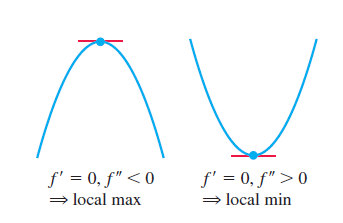
\includegraphics[width = 0.5\linewidth]{Images/second derivative test.png}
\end{figure}

\paragraph{Proof (Statement 2)}
Suppose $f'(c) = 0$ and $f''(x) > 0$. Then, 
\[
    0 < f''(c) = \lim_{x \to c} \frac{f'(x) - f'(c)}{x - c} = \lim_{x \to c} \frac{f'(x)}{x - c} 
\]
\noindent
Let $L = f''(c)$ for $\epsilon = L/2$, $\exists \, \delta > 0$ such that:
\begin{align*} 
     \frac{f'(x)}{x - c} \in (L - \epsilon, L + \epsilon) \textrm{\tab} \forall \, x \in (c - \epsilon, c + \epsilon) \\
     \frac{f'(x)}{x - c} \in (\frac{L}{2}, \frac{3L}{2}) \textrm{\tab} \forall \, x \in (c - \epsilon, c + \epsilon) 
\end{align*}
\[
    \Rightarrow \frac{f'(x)}{x - c} > \frac{L}{2} > 0 \textrm{\tab} \forall \, x \in (c - \delta, c + \delta) 
\]
So, 
\begin{align*} 
    x - c < 0 \Rightarrow f'(x) < 0 \\
    x - c > 0 \Rightarrow f'(x) > 0
\end{align*}
\noindent
Hence, 
\begin{align*} 
    f'(x) < 0 \textrm{ for } (c - \delta, c) \\
    f'(x) > 0 \textrm{ for } (c, c + \delta)
\end{align*}
By corolarry (3) $f$ is decreasing on $[c - \delta, c]$ and increasing on $[c, c + \delta]$. Hence, $f$ 
has a local minimum at $c$.

Statement 1 can be proved by the same method.

\paragraph{Proof (Statement 3)}
Let $f(x) = x^3$, $g(x) = x^4$, $h(x) = -x^4$\\
We have:
\begin{align*} 
     f'(x) = 3x^2 \textrm{\tab} g'(x) = 4x^3 \textrm{\tab} h'(x) = -4x^3 \\
     f''(x) = 6x \textrm{\tab} g''(x) = 12x^2 \textrm{\tab} h''(x) = - 12x^2 \\
\end{align*}
At $x = 0$:
\[
    f'(x) = f''(x) = g'(x) = g''(x) = h'(x) = h''(x)
\]
But, at $x = 0$ (1) $f$ doesn't have a local extremum, (2) $g$ has a local minimum, (3) $h$ has a local maximum.
Hence, when $f''(c) = 0$, $c$ can be an local maximum, minimum, or neither. 
\paragraph{Example} Find all local extrema of $f(x) = x^4 - 4x^3 + 10$!
\begin{itemize} 
    \item \textbf{Step 1} Find all values of $x$ such that $f'(x) = 0$
    \item \textbf{Step 2} Find all values of $f''(x)$ when $f'(x) = 0$
    \item \textbf{Step 3} Apply second derivative test to identify the concavity
    \item \textbf{Step 4} Find $f(x)$ at the local extrema
\end{itemize}
\begin{align*} 
    f'(x) &= 4x^3 - 12x^2 = 4x^2(x - 3) \textrm{\tab} f'(x) = 0 \Rightarrow x = \{0, 3\} \\
    f''(x) &= 12x^2 - 24x \textrm{\tab} f''(0) = 0 \textrm{   } f''(3) = 36 > 0
\end{align*}

So, at $x = 0$, $f(x)$ fails the second derivative test, at $x = 3$, $f''(x) > 0$, and 
$f(x)$ has a local minimum at $x = 3$.  

At $x = 0$, consider $a = -1$ and $b = 1$. $f'(1) < 0$ and $f'(-1) < 0$, so, it is not a local extrema.
\subsection{Concavity and Secant Line}
\begin{theorem}[Concavity and Secant Lines]
    Let $f$ be continuous on $[a, b]$ and differentiable on $(a, b)$.
    \begin{enumerate} 
        \item If $f$ is \textbf{concave down} on $(a, b)$, then the graph of $f$ lies \textbf{above} the secant line joining $(a, f(a))$ and $(b, f(b))$ on $(a, b)$.
        \item  If $f$ is \textbf{concave up} on $(a, b)$, then the graph of $f$ lies \textbf{below} the secant line joining $(a, f(a))$ and $(b, f(b))$ on $(a, b)$.
    \end{enumerate}
\end{theorem}

\subsection{Concavity and Tangent Line}
\begin{theorem}[Concavity and Tangent Lines]
    Let $f$ be continuous on $[a, b]$ and differentiable on $(a, b)$.
    \begin{enumerate} 
        \item If $f$ is \textbf{concave down} on $(a, b)$, then $\forall \, c \in (a, b)$, the tangent line of $f$ at $c$ lies \textbf{above} the graph of $y = f(x)$.
        \item  If $f$ is \textbf{concave up} on $(a, b)$, then $\forall \, c \in (a, b)$, the tangent line of $f$ at $c$ lies \textbf{below} the graph of $y = f(x)$.
    \end{enumerate}
\end{theorem}

\section{Graph Sketching}
Important things to sketch a graph: domain, symmetry, critical points, interval of monotonicity, points of inflection,
intervals of concavity, asymptotes, and x-y intercepts.

\paragraph{Example} Graph the function
\[
    f(x) = \frac{x^2 + 4}{2x} 
\]
(1) Domain = $(-\infty, 0) \cup (0, \infty)$ \\
(2) Symmetry \\
\begin{itemize} 
     \item Odd function/ symmetry on origin if $f(-x) = - f(x)$
     \item Even function / symmetry along y axis if $f(-x) = f(x)$
\end{itemize}

\[
    f'(x) = \frac{( - x)^2 + 4}{ - 2x} = - (\frac{x^2 + 4}{2x}) = - f(x) 
\]
Hence $f(x)$ is an odd function \\ \\
(3) Critical points
\[
    f'(x) = \frac{x^2 - 4}{2x^2} \textrm{\tab} f'(x) = 0 \Rightarrow x = {-2, 2} 
\]
So, $+++|-2|---|\,0\,|---|\,2\,|+++$, 
Minimum point at 2, and maximum point at -2. \\ \\
(4) Point of Inflection
\[
    f''(x) = 4x^{ - 3} \textrm{\tab} f''(x) > 0 \; \forall x > 0 \textrm{ and } f''(x) < 0 \; \forall x < 0
\]
Hence, $f$ concave down on $(- \infty, 0)$  $f$ concave up on $(0, \infty)$ and no point of inflection. \\ \\
(5) Asymptotes \\
Oblique asymptote: $y = Ax + B$
\[
    A = \lim_{x \to \infty} \frac{f(x)}{x} = \frac{x^2 + 4}{2x^2} = \frac{1}{2} 
\]

\[
    B = \lim_{x \to \infty} f(x) - A(x)  = \frac{x^2 + 4 - x^2}{2x} = 0 
\]
So, $y = 1/2x$ is an oblique asymptote\\ \\
Vertical Asymptote :
\[
    \lim_{x \to 0^{ +}} f(x) = \infty
\]
Hence, $x = 0$ is a vertical asymptote. \\ \\
(6) x and y intercepts \\
No x and y intercept since $x, y \neq 0$

\begin{figure}[h!]
     \centering
     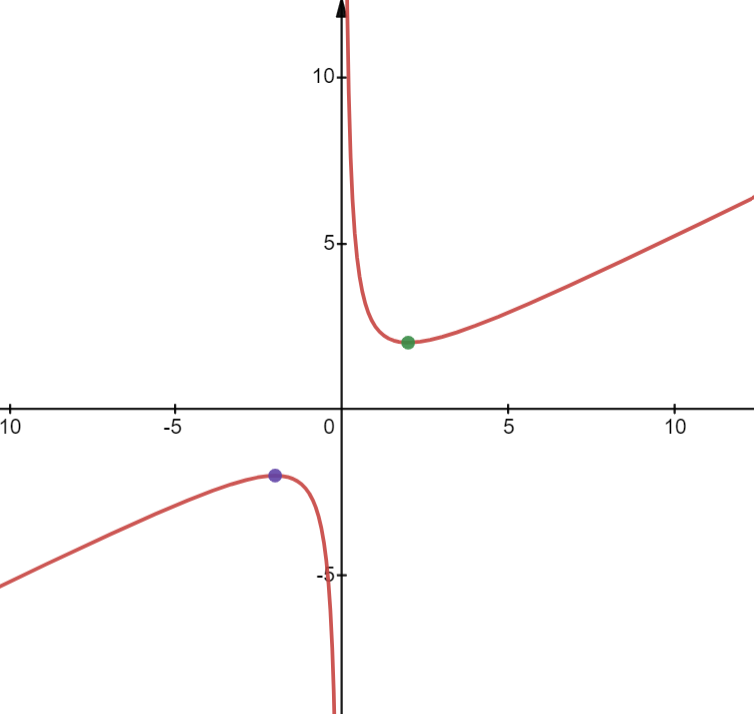
\includegraphics[width = 0.5\linewidth]{Images/graph sketching example.png}
     \caption{Graph of $f(x)$}
\end{figure}
\section{Applied Optimization}
\paragraph{Example 1}
rectangle is to be inscribed in a semicircle of radius 2. What is the
largest area the rectangle can have, and what are its dimensions?

\paragraph{Example 2}
A man launches his boat from point A on a bank of a straight river, 3 km wide, 
and wants to reach point B, 8 km downstream on the opposite bank, as quickly as possible (see figure). He could row his boat directly across the river to point C 
and then run to B, or he could row directly to B, or he could row to some point D between C and B and then run to B. If he can row 6 km/h and run 8 km/h, where should 
he land to reach B as soon as possible? (We assume that the speed of the water is negligible.) 

\paragraph{Example 3}
Suppose $x$ = number of video game consoles, million units \\
Cost : $C(x) = x^3 - 6x^2 + 15x$ \\
Revenue : $R(x) = 9x$ \\
Profit : $P(x) = R(x) - C(x)$ \\
Find $x$ that maximizes profit, if any.

\section{Newton's Method}
\end{document}